\documentclass[final]{beamer}
\usepackage[orientation=portrait, size=a0, scale=1.4]{beamerposter}

% Theme settings
\usetheme{default}
\usecolortheme{seahorse}

% Color definitions
\definecolor{darkblue}{RGB}{0, 51, 102}
\definecolor{lightgray}{RGB}{230, 230, 230}
\setbeamercolor{title}{fg=darkblue}
\setbeamercolor{block title}{bg=darkblue, fg=white}
\setbeamercolor{block body}{bg=lightgray}

% Graphics path
\usepackage{graphicx}
\graphicspath{{../}}

% Title, author, and institution information
\title{Exploring the Dynamical Evolution of Dark Matter Haloes in Cosmological Simulations}
\author{PremVijay Velmani}
\institute{Inter-University Centre for Astronomy and Astrophysics (IUCAA), Pune}
\date{\today}

\begin{document}

% Begin poster content
\begin{frame}[t]

    % Title block
    \begin{center}
        \vspace{1.5cm} % Adjust for spacing if needed
        \usebeamerfont{title} \textcolor{darkblue}{\Huge \textbf{Interplay of galaxy formation and the evolution of dark matter haloes}} \\
        \vspace{0.5cm}
        \usebeamerfont{author} \LARGE{PremVijay Velmani} \\
        \vspace{0.5cm}
        \usebeamerfont{institute} \Large{Inter-University Centre for Astronomy and Astrophysics (IUCAA), Pune} \\
    \end{center}

    \vspace{1cm} % Add space between title and content
    
    \begin{columns}
        % Column 1: Introduction & Methods
        \begin{column}{0.45\textwidth}
            % Introduction
            \begin{block}{Introduction}
            \begin{itemize}
                \item Dark matter haloes are fundamental structures in the Universe, hosting the formation and evolution of galaxies.
                \item Understanding their nature and evolution is a multi-disciplinary task. 
                \item This research investigates the impact of baryonic astrophysical processes on the relaxation of dark matter profiles in haloes.
            \end{itemize}
            \end{block}

            % Methods
            \begin{block}{Methods}
                \begin{itemize}
                    \item Hydrodynamical simulations: IllustrisTNG, EAGLE, CAMELS.
                    \item Quasi-adiabatic relaxation framework.
                    \item Exploration of astrophysical feedback effects.
                    \item Self-similar spherical models of galaxy formation.
                \end{itemize}
            \end{block}
            
            % Placeholder for figure
            \begin{block}{Figure 1}
                \centering
                % 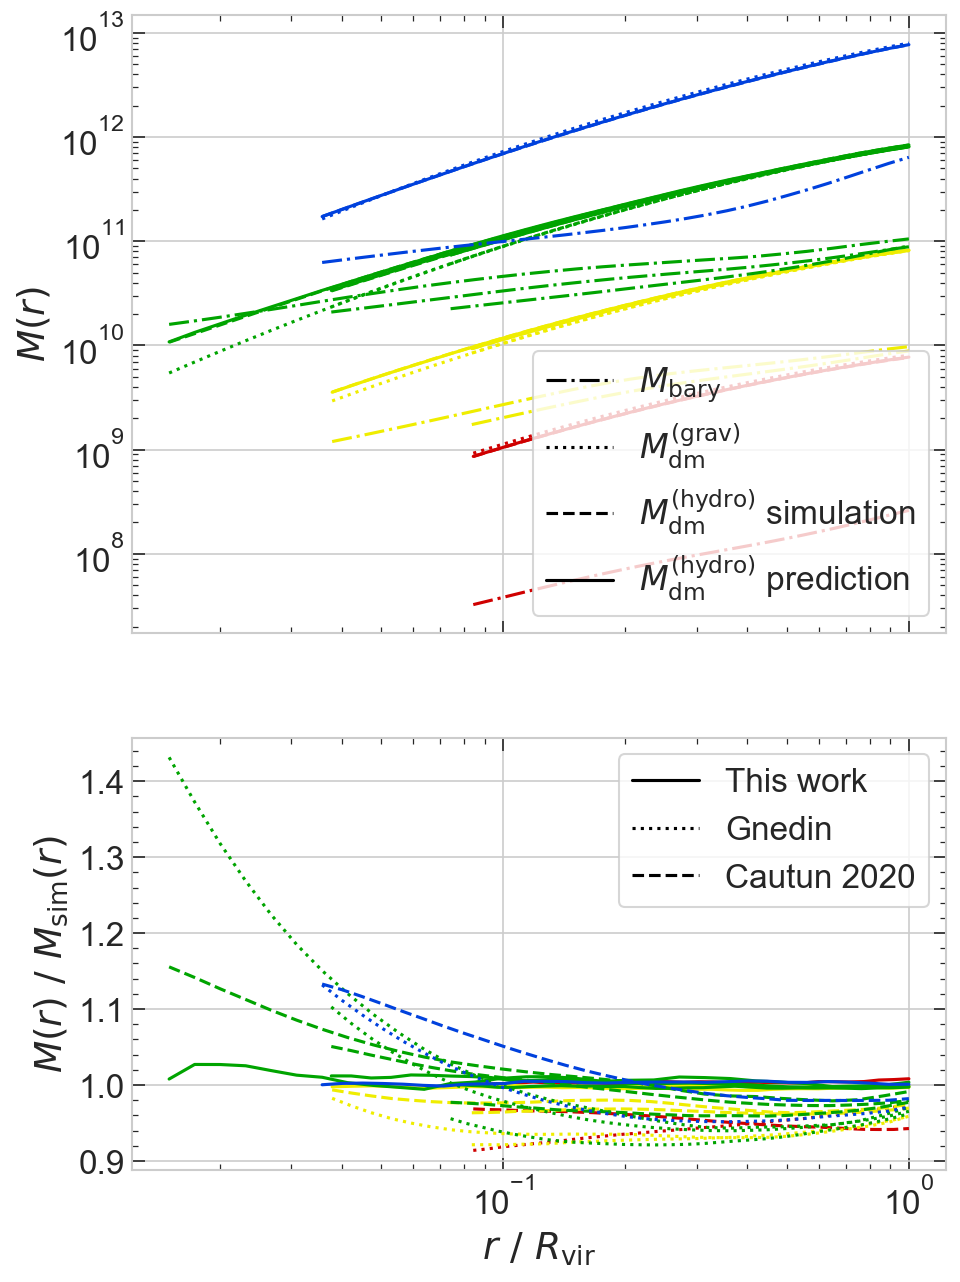
\includegraphics[width=0.9\linewidth]{plots/demo-cautun-gnedin.png} % Add figure path
                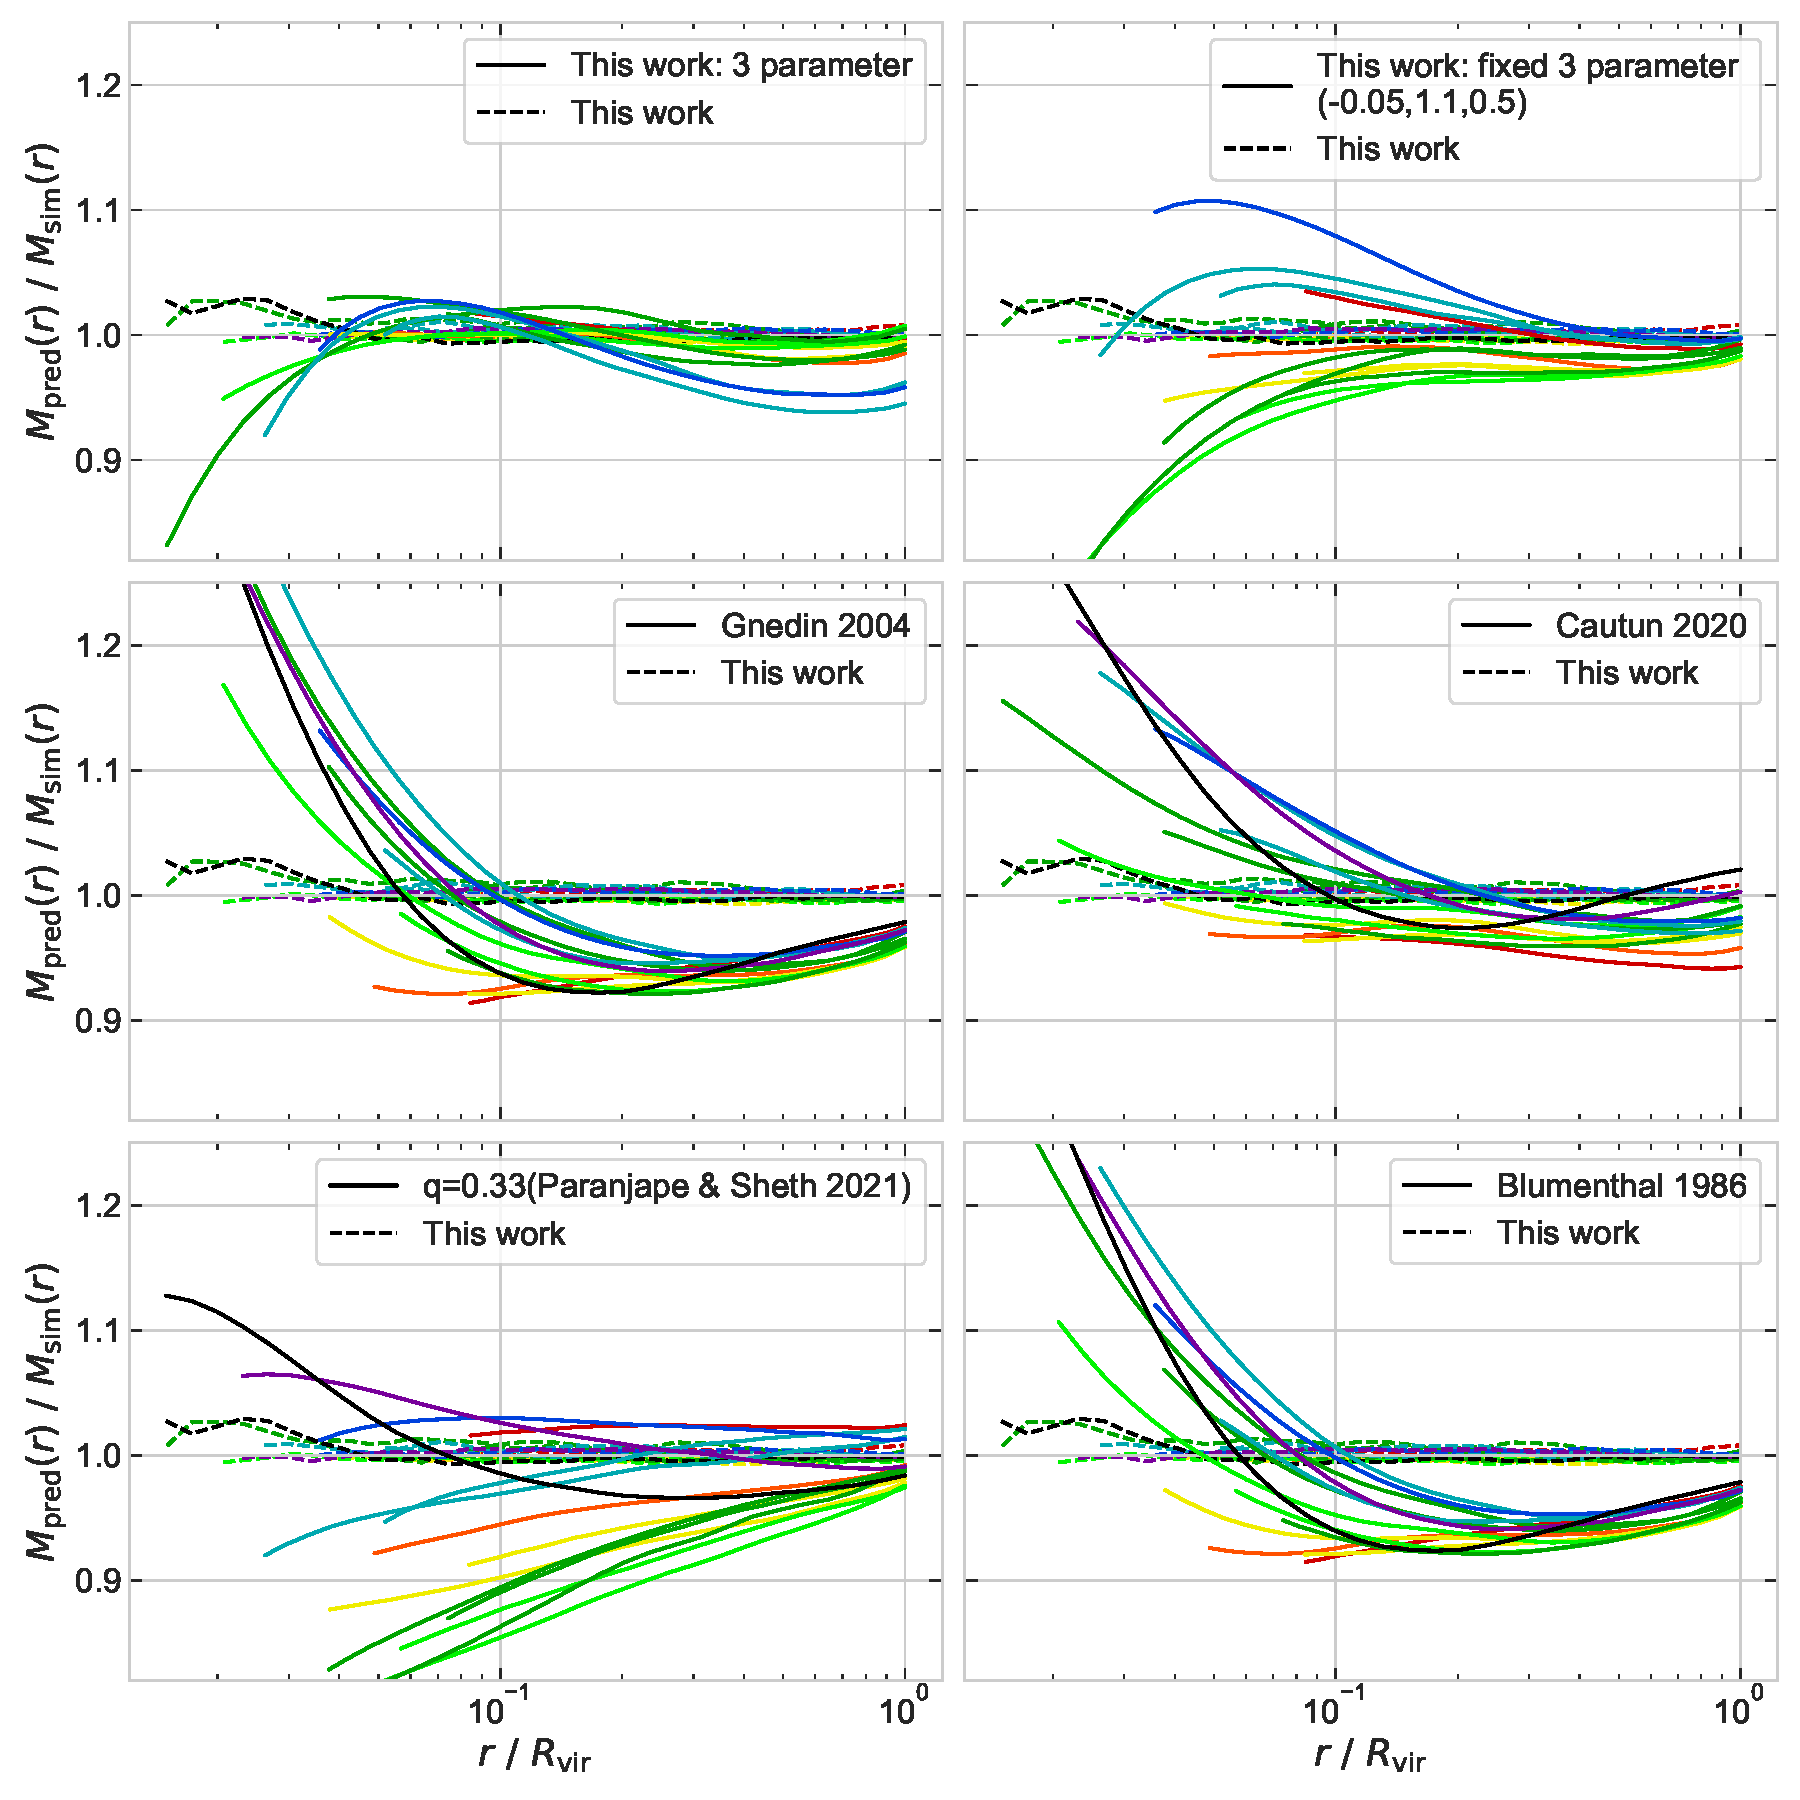
\includegraphics[width=0.9\linewidth]{plots/relxn_model_comparison.pdf} % Add figure path
                \textbf{Simulation of dark matter halo profile.}
            \end{block}
        \end{column}

        % Column 2: Results
        \begin{column}{0.45\textwidth}
            % Results: Part 1
            \begin{block}{Results (Part 1)}
                \textbf{Statistical Response Characterization:}
                \begin{itemize}
                    \item Analysis of halo populations from IllustrisTNG, EAGLE.
                    \item Quasi-adiabatic model fits dark matter relaxation with astrophysical feedback.
                    \item Explicit dependence on halo-centric distance and feedback effects.
                \end{itemize}
            \end{block}
            
            % Placeholder for figure
            \begin{block}{Figure 2}
                \centering
                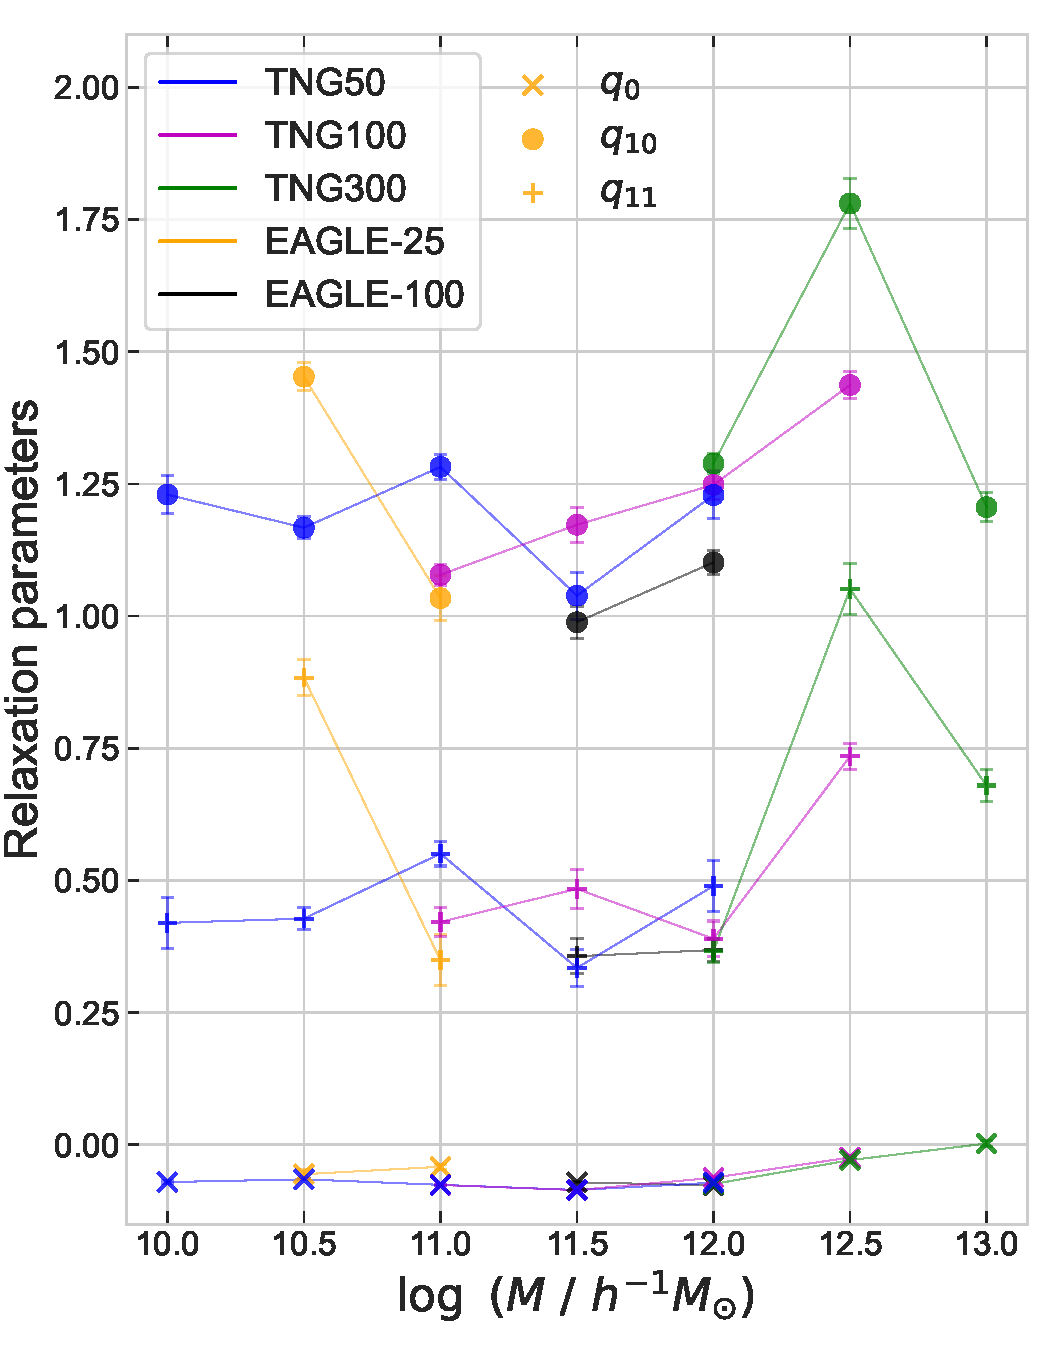
\includegraphics[width=0.6\linewidth]{plots/fit_param_q3s_M_TE.pdf} % Add figure path
                \textbf{Quasi-adiabatic relaxation model.}
            \end{block}

            % Results: Part 2
            \begin{block}{Results (Part 2)}
                \textbf{Epoch-dependent Feedback Effects:}
                \begin{itemize}
                    \item CAMELS simulations: Only feedback outflow energy affects relaxation.
                    \item Effect of feedback on different epochs (e.g., $z=5$ to $z=0$).
                    \item Significant influence of gas equation of state.
                \end{itemize}
            \end{block}
        \end{column}
        \end{columns}
        \begin{columns}
        % Column 3: Self-Similar Model & Conclusions
        \begin{column}{0.45\textwidth}
            % Self-Similar Model
            \begin{block}{Self-Similar Model}
                \textbf{Spherical self-similar gas collapse model:}
                \begin{itemize}
                    \item Simultaneous evolution of gas and dark matter.
                    \item Study of relaxation response with variations in accretion rates and gas equation of state.
                \end{itemize}
            \end{block}

            % Placeholder for figure
            \begin{block}{Figure 3}
                \centering
                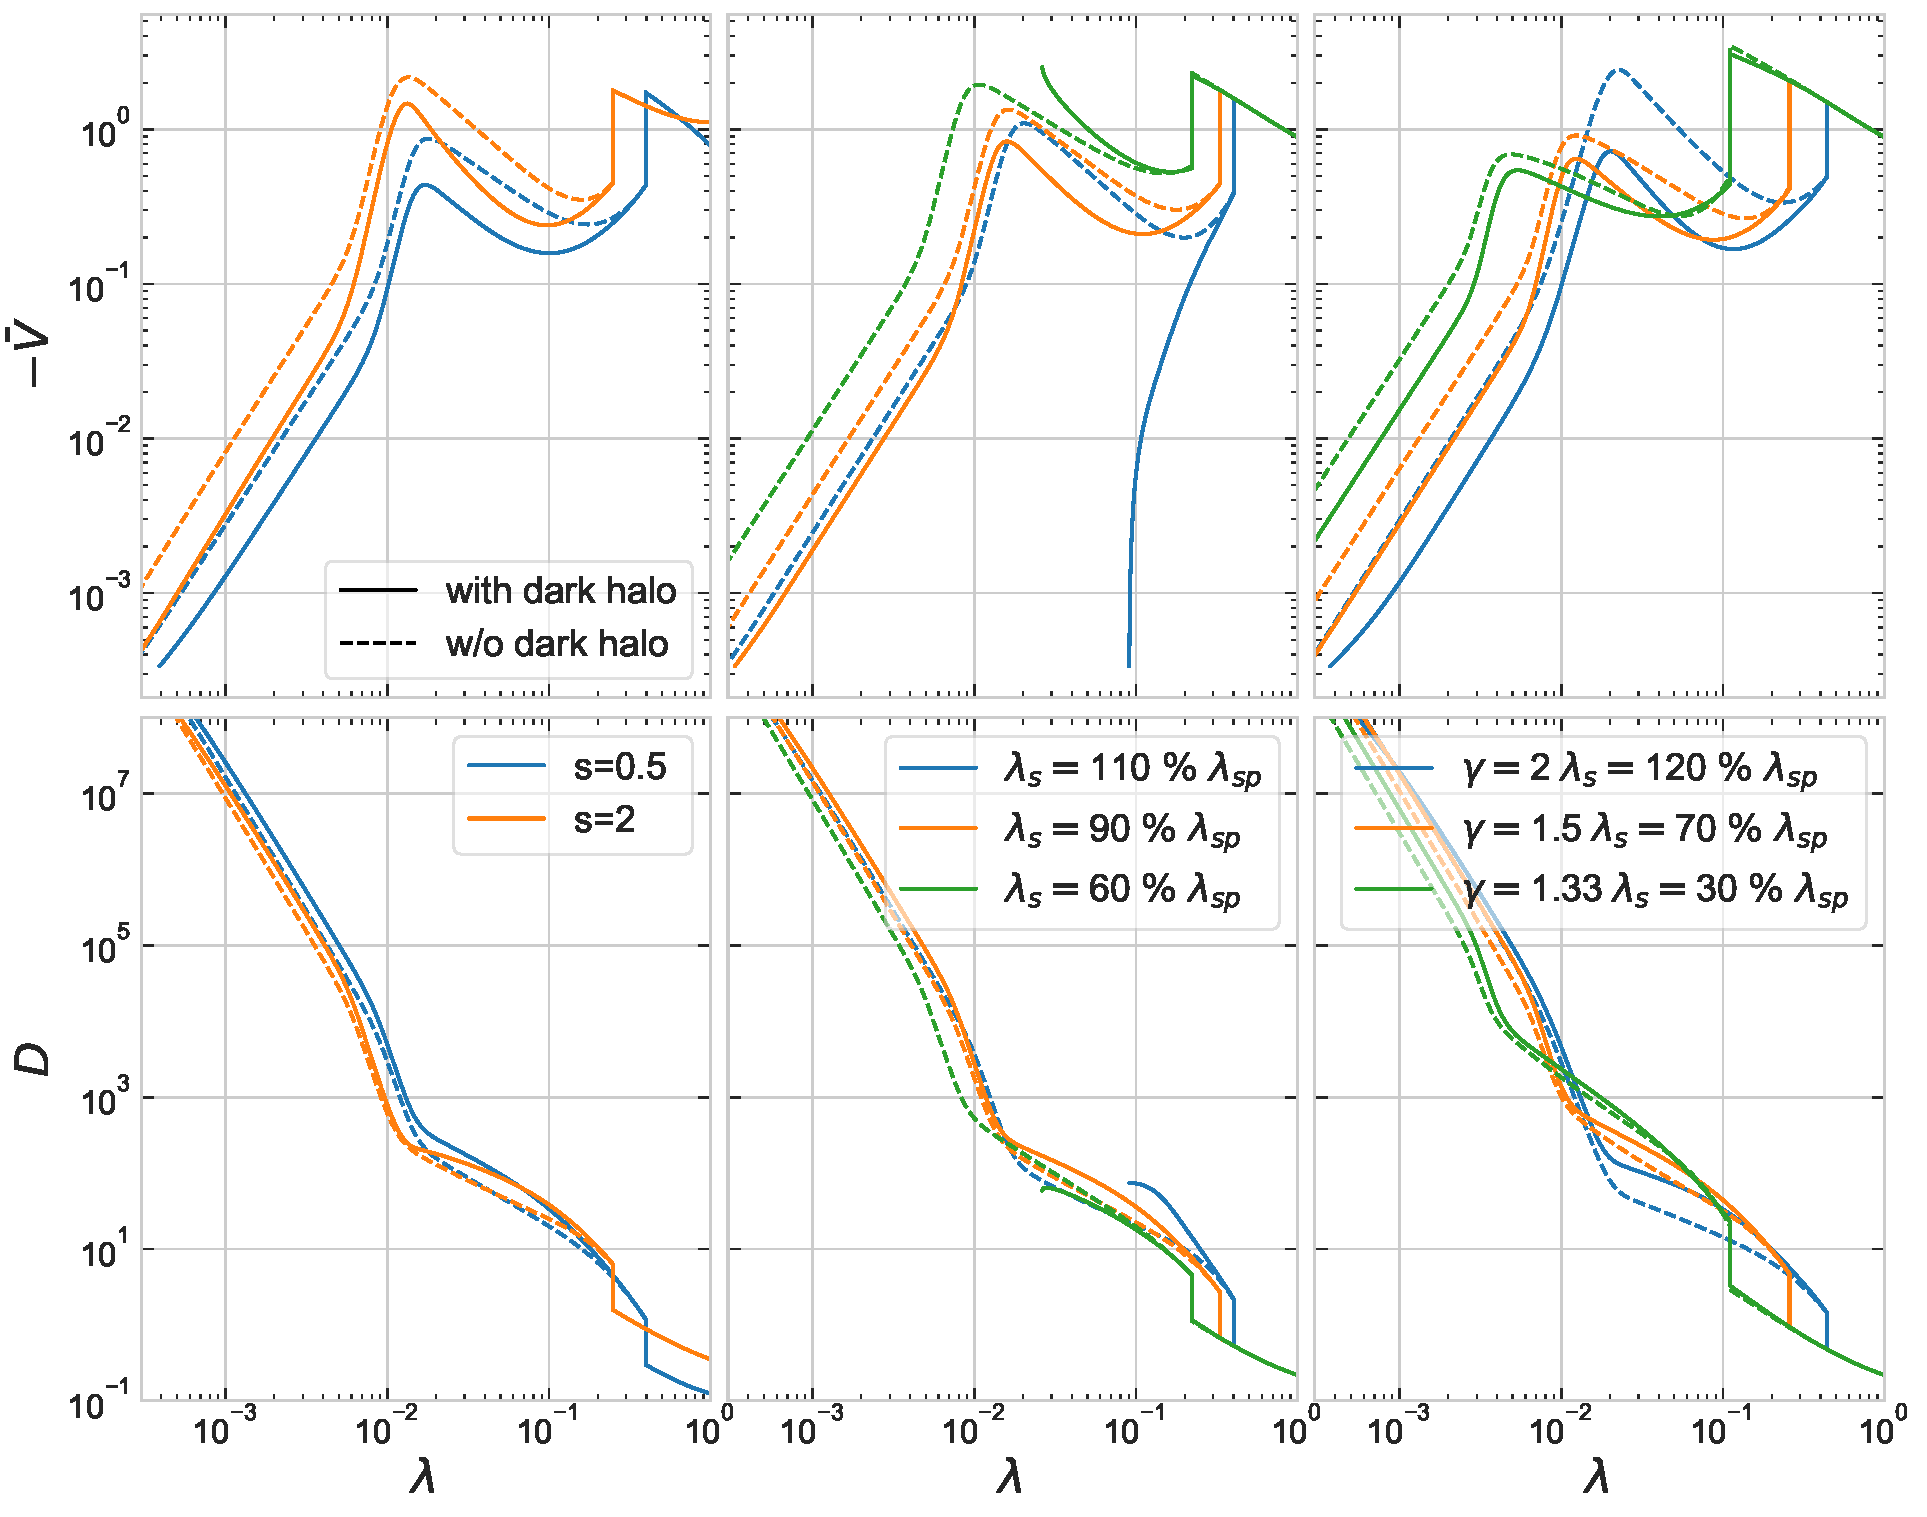
\includegraphics[width=0.9\linewidth]{plots/profiles_gas_w-wo_halo_all.pdf} % Add figure path
                % 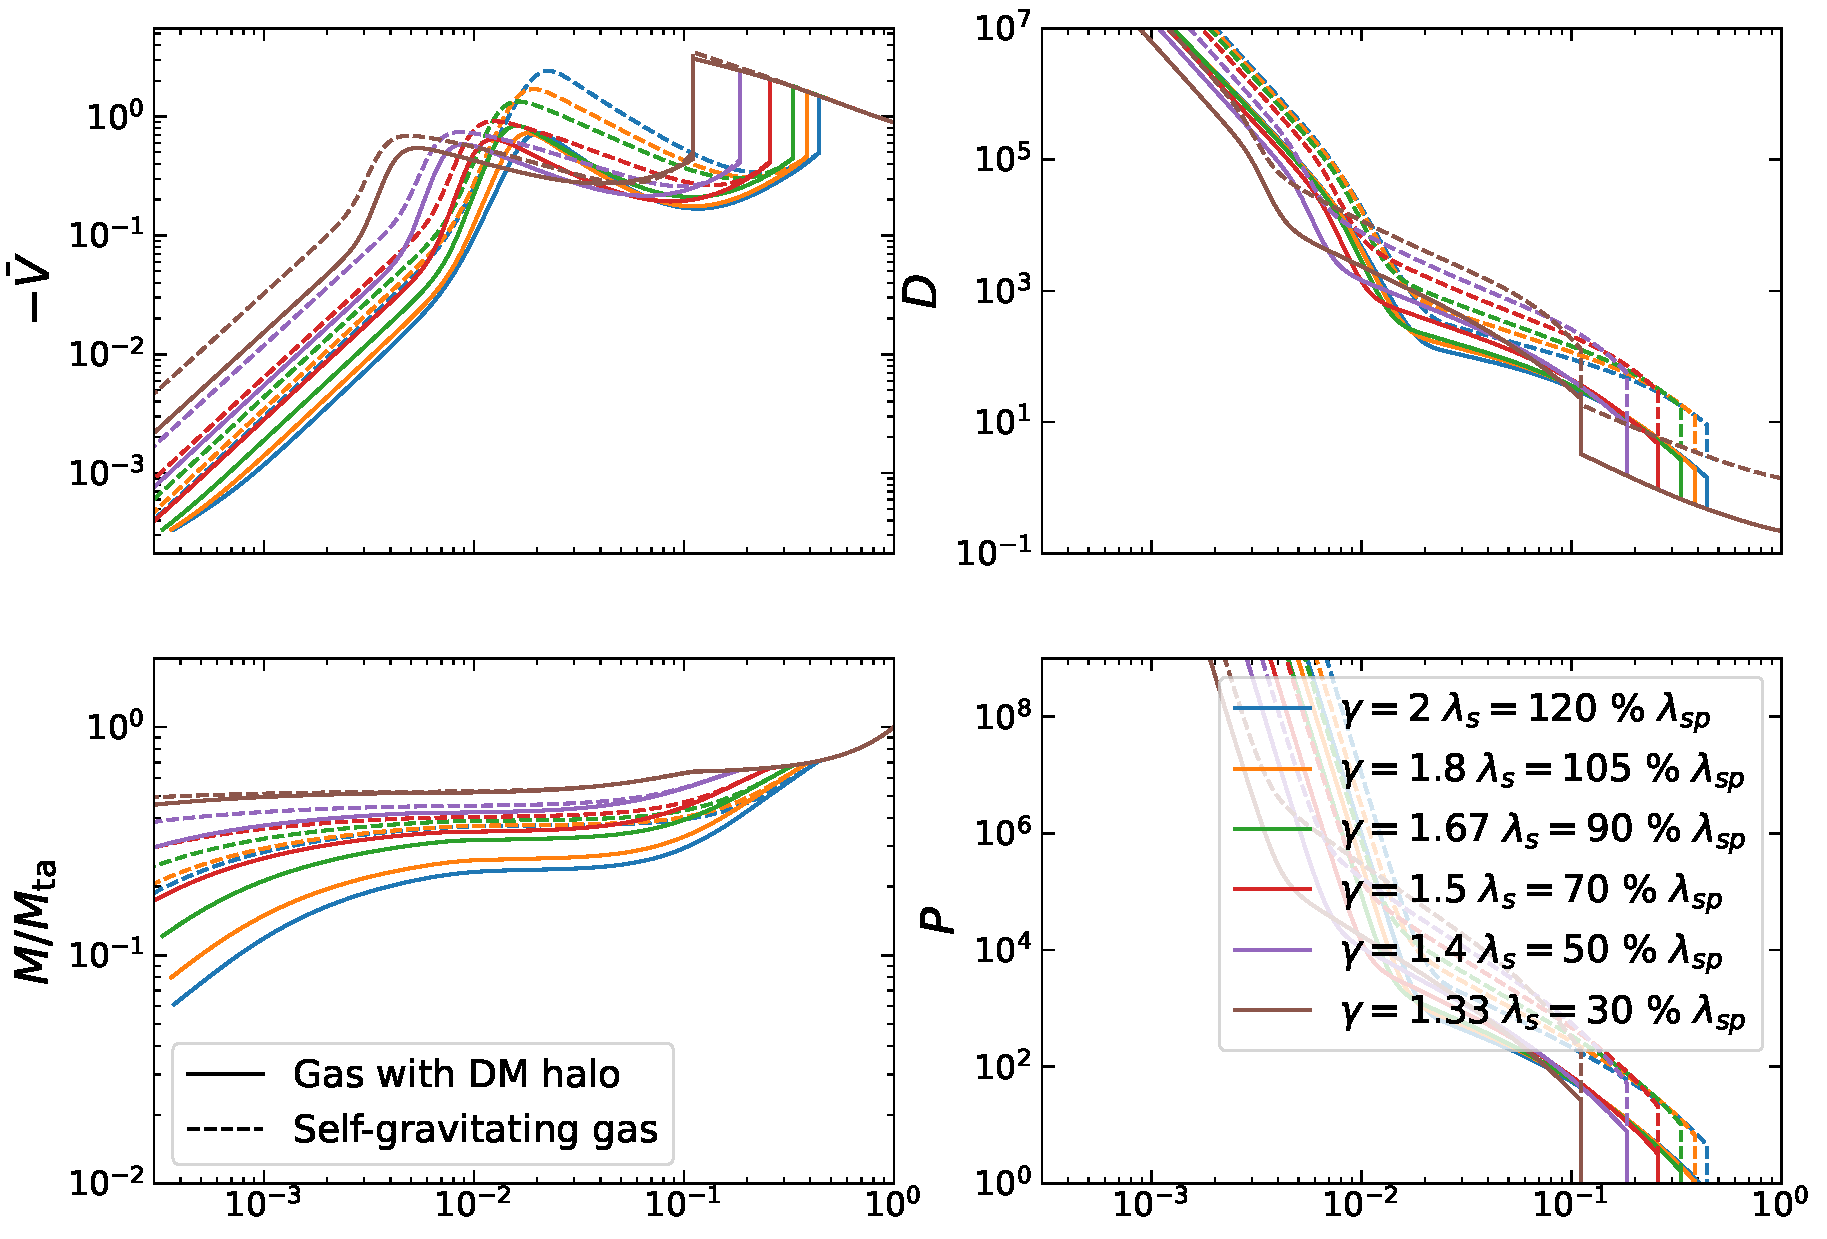
\includegraphics[width=0.9\linewidth]{plots/profiles_gas_shocked_vary-gam.pdf} % Add figure path
                \textbf{Self-similar model: Gas and dark matter profiles.}
            \end{block}
            \end{column}
            \begin{column}{0.45\textwidth}
            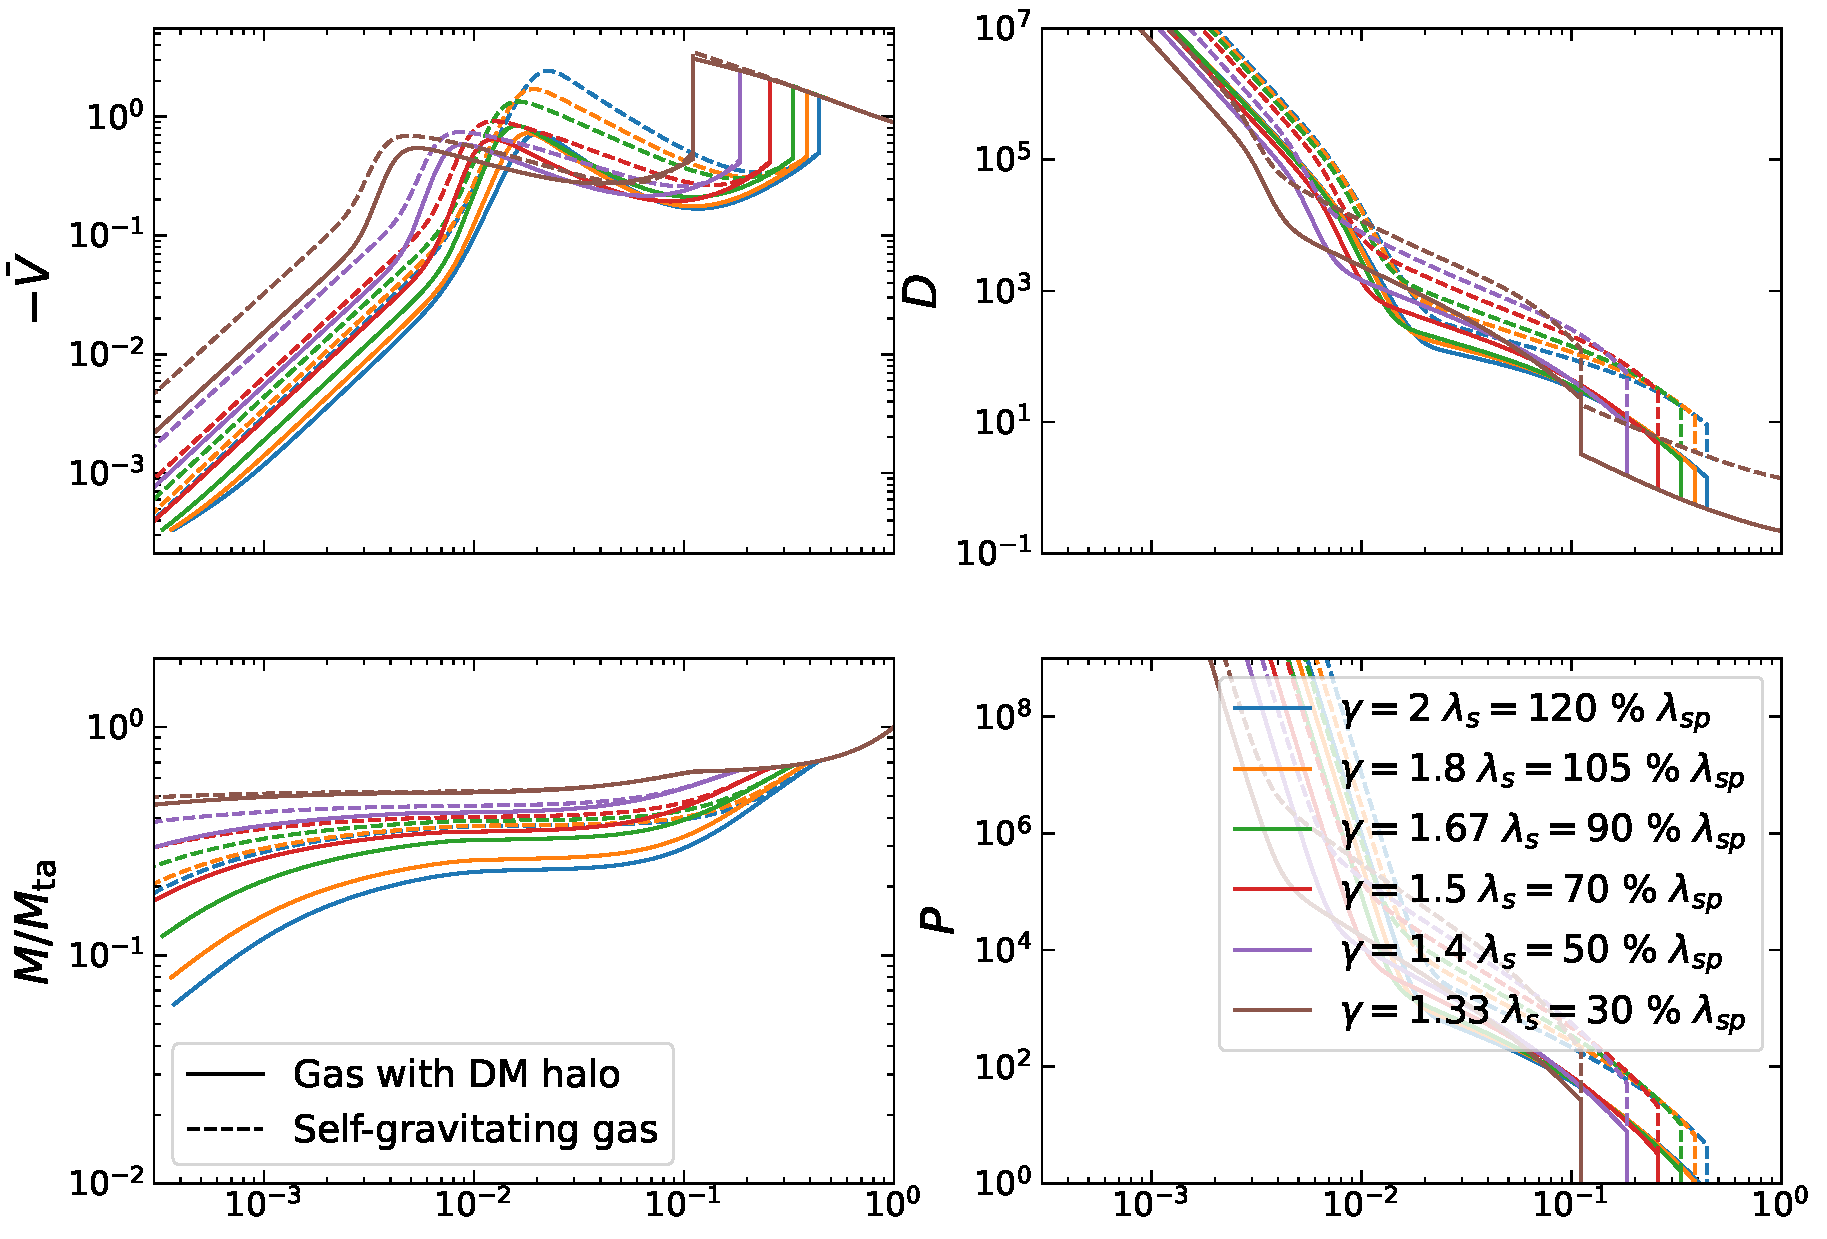
\includegraphics[width=0.9\linewidth]{plots/profiles_gas_shocked_vary-gam.pdf}
            % Conclusions & Future Directions
            \begin{block}{Conclusions and Future Directions}
                \begin{itemize}
                    \item Improved understanding of astrophysical feedback effects on halo relaxation.
                    \item Quasi-adiabatic models applicable across a wide mass range.
                    \item Future work: Explore analytical models and star formation impact.
                \end{itemize}
            \end{block}
            \begin{alertblock}{Summary}
                Thank you
            \end{alertblock}
        \end{column}
    \end{columns}

    % Acknowledgements
    \begin{block}{Acknowledgements}
        This presentation is funded by Inter-University Centre of Astronomy and Astrophysics (IUCAA), Pune.
    \end{block}
    
\end{frame}
\end{document}
